\documentclass{acm_proc_article-sp}
\usepackage{amsmath}
\usepackage{mathtools}
\usepackage[hidelinks]{hyperref}
\usepackage{amssymb}
\usepackage{tikz}
\usepackage{caption}
\usepackage{graphicx}
\graphicspath{{.}}
\usepackage{listings}
\usepackage{verbatim}
\usepackage{xcolor}
\renewcommand\thefootnote{\textcolor{black}{\arabic{footnote}}}
\hypersetup{colorlinks,urlcolor=blue,citecolor=black}
\usepackage[paper=a4paper,
            %includefoot, % Uncomment to put page number above margin
            marginparwidth=10mm,      % Length of section titles
            marginparsep=0.5mm,       % Space between titles and text
            margin=10mm,              % 25mm margins
            includemp]{geometry}

\begin{document}
\title{``Moneyball'' in NBA to predict the performance of the players}
\numberofauthors{3}
\author{
%
% 1st. author
\alignauthor 
Kirill Novik\\
       \email{kirill.novik@colorado.edu}
% 2nd. author
\alignauthor
Krishna Chaitanya Sripada\\
       \email{krishna.sripada@colorado.edu}
% 3rd. author
\alignauthor
Yu-Ching Kuo\\
       \email{yuching.kuo@colorado.edu}
}
\maketitle
\begin{abstract}
``Moneyball'' is a term describing operations in which a team endeavors to analyze the market for players and buy what is undervalued and sell what is overvalued. By using this strategy, NBA managers can decide which player to buy/sell and optimize the performance and the finances of their team. The goal of this project is to analyze the NBA dataset and perform Principal Component Analysis and Discriminant Analysis that help evaluate the performance of the team and the individual players. This analysis can also be used to predict the performance of the team for the coming seasons.
\end{abstract}

\keywords{Data Mining, Principal Component Analysis, Discriminant Analysis, Performance, Prediction} 

\section{Introduction}
Moneyball is a term from the book: ``Moneyball: The Art of Winning an Unfair Game'' which was authored by Michael Lewis in 2003 depicting the story of Oakland Athletics baseball team. The manager Billy Beane of Oakland Athletics applied an analytic approach to look at those players who are undervalued and assemble a competitive team. In the 2002-2003 season, with the Moneyball strategy, Oakland Athletics made to the playoff with only 44 million team salary (125 million for New York Yankees) and also broke the MLB record with 20 straight wins. As a team with small revenue like Oakland Athletics, this is an excellent strategy to compete with those big teams like New York Yankees and Boston Red Socks.

Motivated by the story, we are questioning if the concept of ``moneyball'' can be applied to teams in NBA and if we can devise a statistical approach to find out the undervalued and overvalued NBA players. Additionally, by mining the NBA database, we would like to predict the future performance of the players which can prevent team managers from providing big contracts to those players who may not perform well in the following seasons. Eventually, we are aim at forming an economical and competitive NBA team based on the pattern and the approach we found through data mining.

In an attempt to determine how to evaluate a player's performance, we first need to find out the ``key factors'' for a team to perform well in a specific season. By analyzing the data for the past 30 years, we expect to find some patterns and correlations between the performance and some specific key factors. For example, the good performance may relate to the points, rebounds, assists or even the combinations of those attributes. Once the patterns and the key factors are found, they can be used for evaluating the individual players. However, due to the possible multidimensional key factors we may find, we will utilize multivariate statistical methods including Principal Components Analysis (PCA) and Discriminant Analysis. We begin by constructing a list of variables that we think are important to measure the performance of any individual player, we use PCA on these variables to find new components to describe our data. A key result of PCA is that we reduce the dimensionality of the data set and form a single index. We would also use Discriminant Analysis and the index we found to classify the teams into one of two categories, good performance or bad performance.

\section{Data}
The NBA dataset can be found \href{http://www.basketball-reference.com/teams/}{here}. This dataset comprises of information regarding individual players and the teams. It also consists of information regarding the teams' performance from the previous seasons. The attributes in the data are shown below.

\begin{figure}[!htb]
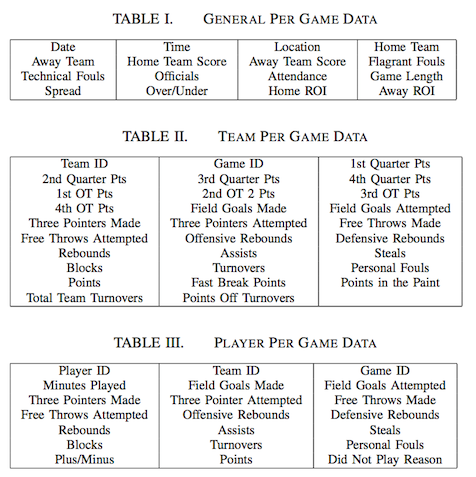
\includegraphics{attributes.png}
\caption{The attributes in the dataset}
\end{figure}

\vspace{12em}
\section{Principal Components Analysis}
When analyzing data with multiple variables, Principal Component Analysis (PCA) can be used to reduce the size of the data set. PCA uses a linear combination of the original correlated variables to form new, uncorrelated variables called principal components. In order to use PCA on the data set, we need to verify the conditions \textbf{normality} and \textbf{dependence} of variables. For each of these conditions, we use hypothesis testing to see if the data meets its criterion. PCA is most effective when the vector of \textit{r} variables of interest has a multivariate normal distribution with mean vector\\ 
\[
\mu=
\begin{bmatrix}
    \mu_{1} \\    
    \mu_{2} \\
    \vdots \\
    \mu_{r}
\end{bmatrix}
\]
and variance-covariance matrix 
\[
\Sigma =
\begin{bmatrix}
    \sigma_{11} & \sigma_{12} & \dots &  \sigma_{1r} \\
    & \sigma_{22} & \dots  & \sigma_{2r} \\
    & & \ddots & \vdots \\
    & & & \sigma_{rr} 
\end{bmatrix}
\]

Once the principal components have been found, they can be identified by carefully interpreting which variables have the greatest contribution to each component. We can test for normality and dependence of variables by using a Q-Q plot where each variables' correlation with its z-score can be calculated and plotted. We are planning to use mlpy  ~\cite{mlpy} package in python for this analysis.

\section{Discriminant Analysis}
The basic goal of discriminant analysis is to project the dataset onto a lower-dimensional space with good class separability in order to avoid overfitting and also reduce computational costs. This analysis can be used to classify the performance of the player/team as good/bad. We are planning to use mlpy  ~\cite{mlpy} package in python for this.

\section{Prediction and Patterns}
From the analysis we are going to find the performance of each player through the index and then use it to evaluate the performance of the teams in the 2015 season. If a specific team scores high from the index of analysis, it means from the prediction point of view, this team should perform well this season. If the team plays well this season, our approach can be validated. On the other hand, if it doesn?t, we need to modify our approach and refine the analysis. We are going to correlate our evaluation with the real performance of the team in NBA 2015 season with a minimum deviation to validate our approach.

Except for the evaluating the performance of a player, we would like to take into account for the possible performance of a player in the following season and fit it into our evaluation. This information is critical for us to avoid providing contracts for those who may not play well in the future. For example, Steve Nash, a two time MVP who was one of the top point guard in the NBA league when he was in Phoenix Suns may be a player who is overvalued by Los Angeles Lakers in 2012. According to the NBA dataset, his average score has been decreasing since 2005 and at the same time he was 37 years old and that is likely to affect his performance. It turned out that he only played 65 out of 164 games for Lakers and was earning 9.1 million per year. From Figure 2, the performance of Steve Nash is decreasing while his salaries stay a constant.

\begin{figure}[!htb]
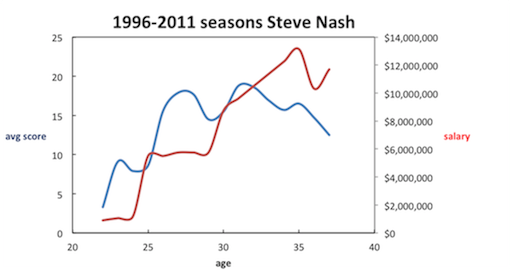
\includegraphics{SN.png}
\caption{The average score vs age for Steve Nash from seasons 1996-2011}
\end{figure}

The approaches such as the Weibull-Gama Statistical Timing Model  ~\cite{wgstm} can be used to forecast the player's future performance. It was shown to be a great metric in part because it is time dependent. However, the approach should be further validated again since only one season (2010-2011) is shown to be accurate and the prediction for LeBron James is not accurate for the recent seasons (2012-2015). The average score of LeBron James is shown in Figure 3 which is totally different from the prediction from the paper  ~\cite{wgstm} as shown in Figure 4.

\begin{figure}[!htb]
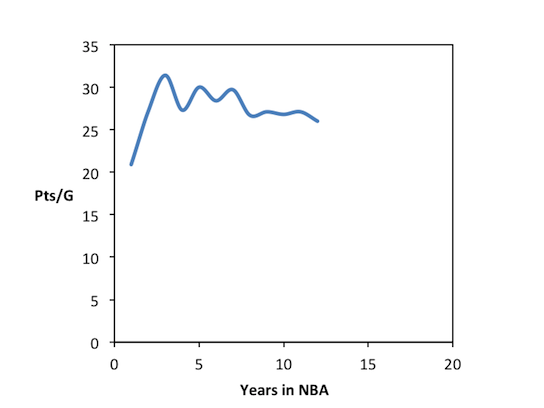
\includegraphics{Fig3.png}
\caption{The actual performance of LeBron James}
\end{figure}

\begin{figure}[!htb]
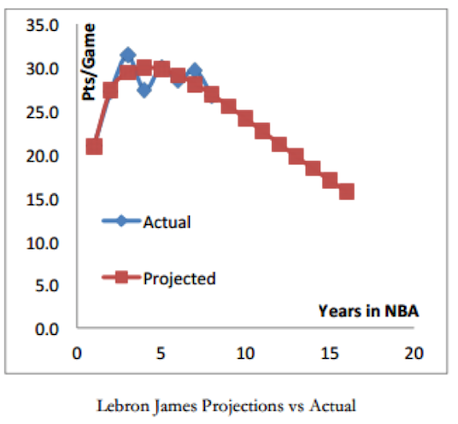
\includegraphics{Fig4.png}
\caption{The prediction of LeBron James's performance in the literature  ~\cite{wgstm}}
\end{figure}

Few of the patterns we are looking at is to find the variation of the average score versus the age of the player and we expect the score to drop as the age of the player increases. Also, we could try to understand the performance of the team by plotting the points scored across all the seasons they have played. The figures 5 and 6 show the comparison between points for all the seasons the Denver Nuggets and the Atlanta Hawks teams have played in.

\begin{figure}[!htb]
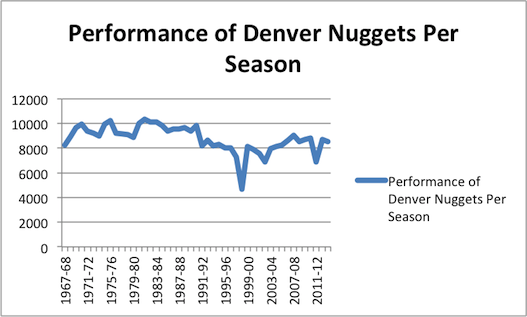
\includegraphics{DN.png}
\caption{Points earned by the team Denver Nuggets per season}
\end{figure}

\begin{figure}[!htb]
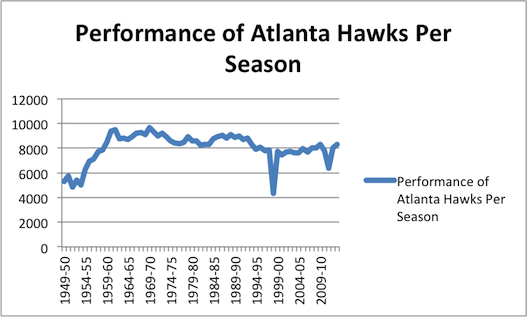
\includegraphics{ATH.png}
\caption{Points earned by the team Atlanta Hawks per season}
\end{figure}

From this we could understand that the Denver Nuggets had a better season than Atlanta Hawks as reflected by the points.

\section{Conclusion}
In order to get an idea of which team or player is performing well, we will use PCA to reduce the dimensionality of our data. We would like to build a model using the discriminant analysis which makes use of a linear discriminant function that helps predict the performance of the team/player based on the attributes available in the data set and this analysis should help decide which player to buy/sell and manage the finances of the team but at the same time improve the performance of the team. This model would be able to predict the performance of the team in the future seasons as well.

\begin{thebibliography}{}
\bibitem{mlpy}D. Albanese, R. Visintainer, S. Merler, S. Riccadonna, G. Jurman, C. Furlanello. mlpy: Machine Learning Python, 2012.
\bibitem{wgstm}Douglas Hwang. Forecasting NBA Player Performance using a Weibull-Gamma Statistical Timing Model, 2012.
\setlength{\itemindent}{0.13in}
\bibitem{CP}Muthu Alagappan. Redefining the Positions in Basketball, 2012.
\end{thebibliography}

\end{document}
